% This file was converted to LaTeX by Writer2LaTeX ver. 1.0.2
% see http://writer2latex.sourceforge.net for more info
\documentclass{tufte-book}

\usepackage[utf8]{inputenc}
\usepackage[T1]{fontenc}
\usepackage[spanish]{babel}
\usepackage{amsmath}
\usepackage{upgreek}
\usepackage{amssymb,amsfonts,textcomp}
\usepackage{array}
\usepackage{supertabular}
\usepackage{hhline}
\usepackage{graphicx}

\makeatletter
\newcommand\arraybslash{\let\\\@arraycr}
\makeatother
\setlength\tabcolsep{1mm}
\renewcommand\arraystretch{1.3}
\newcommand\wideslash[2]{{}^{#1}/_{#2}}
\newcommand\normalsubformula[1]{\text{\mathversion{normal}$#1$}}
\author{SOL}
\date{2011-09-01}

\hypersetup{colorlinks}% uncomment this line if you prefer colored hyperlinks (e.g., for onscreen viewing)

%%
% Book metadata
\title{Representaciónes \\ Cartográficas \thanks{Datum}}
\author[Miguel Starobinsky \ Javier Clavijo]{Miguel Starobinsky \ Javier Clavijo}
\publisher{Publisher of This Book}

%%
% If they're installed, use Bergamo and Chantilly from www.fontsite.com.
% They're clones of Bembo and Gill Sans, respectively.
%\IfFileExists{bergamo.sty}{\usepackage[osf]{bergamo}}{}% Bembo
%\IfFileExists{chantill.sty}{\usepackage{chantill}}{}% Gill Sans

%\usepackage{microtype}

%%
% Just some sample text
\usepackage{lipsum}

%%
% For nicely typeset tabular material
\usepackage{booktabs}

%%
% For graphics / images
\usepackage{graphicx}
\setkeys{Gin}{width=\linewidth,totalheight=\textheight,keepaspectratio}
\graphicspath{{graphics/}}

% The fancyvrb package lets us customize the formatting of verbatim
% environments.  We use a slightly smaller font.
\usepackage{fancyvrb}
\fvset{fontsize=\normalsize}

%%
% Prints argument within hanging parentheses (i.e., parentheses that take
% up no horizontal space).  Useful in tabular environments.
\newcommand{\hangp}[1]{\makebox[0pt][r]{(}#1\makebox[0pt][l]{)}}

%%
% Prints an asterisk that takes up no horizontal space.
% Useful in tabular environments.
\newcommand{\hangstar}{\makebox[0pt][l]{*}}

%%
% Prints a trailing space in a smart way.
\usepackage{xspace}

%%
% Some shortcuts for Tufte's book titles.  The lowercase commands will
% produce the initials of the book title in italics.  The all-caps commands
% will print out the full title of the book in italics.
\newcommand{\vdqi}{\textit{VDQI}\xspace}
\newcommand{\ei}{\textit{EI}\xspace}
\newcommand{\ve}{\textit{VE}\xspace}
\newcommand{\be}{\textit{BE}\xspace}
\newcommand{\VDQI}{\textit{The Visual Display of Quantitative Information}\xspace}
\newcommand{\EI}{\textit{Envisioning Information}\xspace}
\newcommand{\VE}{\textit{Visual Explanations}\xspace}
\newcommand{\BE}{\textit{Beautiful Evidence}\xspace}

\newcommand{\TL}{Tufte-\LaTeX\xspace}

% Prints the month name (e.g., January) and the year (e.g., 2008)
\newcommand{\monthyear}{%
  \ifcase\month\or Enero\or Febrero\or Marzo\or Abril\or Mayo\or Junio\or
  Julio\or Agosto\or Septiembre\or Octubre\or Noviembre\or
  Diciembre\fi\space\number\year
}


% Prints an epigraph and speaker in sans serif, all-caps type.
\newcommand{\openepigraph}[2]{%
  %\sffamily\fontsize{14}{16}\selectfont
  \begin{fullwidth}
  \sffamily\large
  \begin{doublespace}
  \noindent\allcaps{#1}\\% epigraph
  \noindent\allcaps{#2}% author
  \end{doublespace}
  \end{fullwidth}
}

% Inserts a blank page
%\newcommand{\blankpage}{\newpage\hbox{}\thispagestyle{empty}\newpage}

\usepackage{units}

% Typesets the font size, leading, and measure in the form of 10/12x26 pc.
\newcommand{\measure}[3]{#1/#2$\times$\unit[#3]{pc}}

% Macros for typesetting the documentation
\newcommand{\hlred}[1]{\textcolor{Maroon}{#1}}% prints in red
\newcommand{\hangleft}[1]{\makebox[0pt][r]{#1}}
\newcommand{\hairsp}{\hspace{1pt}}% hair space
\newcommand{\hquad}{\hskip0.5em\relax}% half quad space
\newcommand{\TODO}{\textcolor{red}{\bf TODO!}\xspace}
\newcommand{\na}{\quad--}% used in tables for N/A cells
\providecommand{\XeLaTeX}{X\lower.5ex\hbox{\kern-0.15em\reflectbox{E}}\kern-0.1em\LaTeX}
\newcommand{\tXeLaTeX}{\XeLaTeX\index{XeLaTeX@\protect\XeLaTeX}}
% \index{\texttt{\textbackslash xyz}@\hangleft{\texttt{\textbackslash}}\texttt{xyz}}
\newcommand{\tuftebs}{\symbol{'134}}% a backslash in tt type in OT1/T1
\newcommand{\doccmdnoindex}[2][]{\texttt{\tuftebs#2}}% command name -- adds backslash automatically (and doesn't add cmd to the index)
\newcommand{\doccmddef}[2][]{%
  \hlred{\texttt{\tuftebs#2}}\label{cmd:#2}%
  \ifthenelse{\isempty{#1}}%
    {% add the command to the index
      \index{#2 command@\protect\hangleft{\texttt{\tuftebs}}\texttt{#2}}% command name
    }%
    {% add the command and package to the index
      \index{#2 command@\protect\hangleft{\texttt{\tuftebs}}\texttt{#2} (\texttt{#1} package)}% command name
      \index{#1 package@\texttt{#1} package}\index{packages!#1@\texttt{#1}}% package name
    }%
}% command name -- adds backslash automatically
\newcommand{\doccmd}[2][]{%
  \texttt{\tuftebs#2}%
  \ifthenelse{\isempty{#1}}%
    {% add the command to the index
      \index{#2 command@\protect\hangleft{\texttt{\tuftebs}}\texttt{#2}}% command name
    }%
    {% add the command and package to the index
      \index{#2 command@\protect\hangleft{\texttt{\tuftebs}}\texttt{#2} (\texttt{#1} package)}% command name
      \index{#1 package@\texttt{#1} package}\index{packages!#1@\texttt{#1}}% package name
    }%
}% command name -- adds backslash automatically
\newcommand{\docopt}[1]{\ensuremath{\langle}\textrm{\textit{#1}}\ensuremath{\rangle}}% optional command argument
\newcommand{\docarg}[1]{\textrm{\textit{#1}}}% (required) command argument
\newenvironment{docspec}{\begin{quotation}\ttfamily\parskip0pt\parindent0pt\ignorespaces}{\end{quotation}}% command specification environment
\newcommand{\docenv}[1]{\texttt{#1}\index{#1 environment@\texttt{#1} environment}\index{environments!#1@\texttt{#1}}}% environment name
\newcommand{\docenvdef}[1]{\hlred{\texttt{#1}}\label{env:#1}\index{#1 environment@\texttt{#1} environment}\index{environments!#1@\texttt{#1}}}% environment name
\newcommand{\docpkg}[1]{\texttt{#1}\index{#1 package@\texttt{#1} package}\index{packages!#1@\texttt{#1}}}% package name
\newcommand{\doccls}[1]{\texttt{#1}}% document class name
\newcommand{\docclsopt}[1]{\texttt{#1}\index{#1 class option@\texttt{#1} class option}\index{class options!#1@\texttt{#1}}}% document class option name
\newcommand{\docclsoptdef}[1]{\hlred{\texttt{#1}}\label{clsopt:#1}\index{#1 class option@\texttt{#1} class option}\index{class options!#1@\texttt{#1}}}% document class option name defined
\newcommand{\docmsg}[2]{\bigskip\begin{fullwidth}\noindent\ttfamily#1\end{fullwidth}\medskip\par\noindent#2}
\newcommand{\docfilehook}[2]{\texttt{#1}\index{file hooks!#2}\index{#1@\texttt{#1}}}
\newcommand{\doccounter}[1]{\texttt{#1}\index{#1 counter@\texttt{#1} counter}}

% Generates the index
\usepackage{makeidx}
\makeindex


\begin{document}

\maketitle

\chapter{La Figura de La tierra}

\newthought{El concepto de \textbf{Datum}} atraviesa los campos de la geodesia y
las representaciones cartográficas y se encuentra en la base de la construcción
de cualquier clase de documento geográfico.
Sin embago, no es posible darle una definición unívoca al término, siendo que se
lo utiliza tanto formal como informalmente para designar una multiplicidad de
conceptos relacionados.
Desarollaremos los conceptos necesarios a través del planteo de lo que podemos llamar
como \guillemotleft problema del datum \guillemotright, incluyendo al mismo tiempo
los conceptos relacionados de \textit{sistema de referencia} y \textit{marco de referencia}.

\section{El problema del datum: Enunciado}

\newthought{\guillemotleft Encuentre Un Método Sistemático } que le permita representar
puntos con exactitud arbitraria sobre la superficie de la tierra partiendo solo de datos
susceptibles de ser medidos desde la misma. \guillemotright

Se nos pide encontrar un método para ubicar puntos sobre la tierra con exactitud
arbitraria. Esto implica definir un sistema de coordenadas que sea válido para cualquier
punto sobre la tierra.

La solución intuitiva a este problema es la definición de un sistema de coordenadas
cartesianas geocéntricas. Sin embargo, esta propuesta se torna inviable si consideramos
que la orientación con respecto a estos ejes no es \textit{a-priori} accesible
desde un punto arbitrario de la superficie terrestre.

Esto nos lleva a considerar la pregunta que sigue, relacionada al enunciado del problema.
¿Cuales son los datos susceptibles de ser medidos desde la superficie terrestre?

\subsection{El sistema de coordenadas local}

Un observador ubicado en la superficie terrestre es capaz de medir distintas cantidades en
forma directa.

En primer lugar, puede medir la orientación de la línea de plomada, o vertical del lugar,
que corresponde a una linea de fuerza del campo gravitatorio terrestre.

Por otro lado, es capaz de identificar una superficie horizontal, es decir materializar un
plano perpendicular a la vertical del lugar, o dicho de otro modo, un plano tangente a la
superficie equipotencial del campo gravitatorio terrestre que pasa por el punto en cuestion.

Para hacerse una idea más gráfica de estos conceptos, puede notarse que, de suponerse una tierra
esférica, homogenea e irrotacional, las superficies equipotenciales constituyen superficies de
esferas concentricas, y las lineas verticales son radios que unen el punto observado con el
centro de la tierra.

\begin{figure}
  \label{fig:equipotenciales}
  \caption{Representación esquemática de superficies equipotenciales y linea de plomada}
  \includegraphics{./imgs/Equipotenciales.jpg}
\end{figure}

A partir de estos datos observados, podría plantearse un sistema de coordenadas locales a ese
punto. Por ejemplo, se define una terna cartesiana con el eje \textbf{z} alineado a la vertical del lugar
y el plano \textbf{tx} correspondiendo al plano horizontal. Sin embargo, aun necesitamos agregar
información al sistema para dejar fija la orientación del eje \textbf{x}. 

\begin{marginfigure}
  \label{fig:plomadayhorizonte}
  \caption{Terna cartesiana referida a la vertical del lugar.}
  \includegraphics{./imgs/PlomadaHorizonte.jpg}
\end{marginfigure}

Podriamos fijar una orientación arbitraria del eje x, y, a partir de esta construcción, realizar
mediciones de ángulos horizontales y distancias. Esto es lo que hacemos al utilizar un teodolito
o estación total.

Ahora bien, el sistema propuesto no es una solución global a nuestro problema. Un observador que
realizara mediciones en este sistema notará que la vertical de un punto arbitrario distinto del
origen no es perpendicular al plano \textbf{xz}, siendo este efecto más exagerado a medida que
nos alejamos del origen.

Si por un momento hacemos la suposicion de que el observador puede materializar un plano horizontal
arbitrariamente grande, vemos que, si se aleja a suficiente distancia del origen, y mide ángulos
entre dicho plano y distintas líneas de plomada locales, llegará a la ineludible conclución de que
está trabajando sobre una superficie que no es plana. Si el observador fue suficientemente cuidadoso
al medir las distancias y orientaciones en cada punto hacia y desde el punto origen, estará en condiciones
de inferir que está trabajando sobre una superficie aproximadamente esférica, y podrá estimar el radio.

Este es el experimento de eratóstenes. En su caso, la materialización del plano arbitrariamente grande
la logró utilizando un plano perpendicular a la dirección que une al observador con el sol, haciendo la
razonable suposición de que el sol está suficientemente lejos para considerar esta dirección inmutable.
Luego, utilizó la sombra en un pozo para sincronizarce con el momento en que su dirección de referencia
coincidia con la vertical de un lugar, y la sombra de una columna o varilla, para medir el ángulo formado
con la vertical en otro lugar. Los puntos flojos de este experimento radican en la medición de distancia,
calculada a partir de un tiempo de viaje, y en el error producido en la medicion del tiempo por los medios
de la época.

\begin{marginfigure}
  \label{fig:eratostenes}
  \caption{Esquema del experimento de Eratóstenes.}
  \includegraphics{./imgs/Eratostenes.png}

\end{marginfigure}

\subsection{Referirse a puntos lejanos: Observaciones Astronómicas}

\newthought{Las estrellas representan una referencia} de inestimable utilidad cuando nos proponemos
medir puntos sobre la tierra. Su importancia es evidente toda vez que vemos que la única
referencia intuitiva con la que contamos, es decir, la verticalidad, no constituye un eje constante
sino que nos da una dirección que varia dependiendo de nuestra ubicación.

Es por eso, que, para seguir considerando la información con la que contamos, que podemos introducir
la latitud astronómica y el azimut astronómico.

No entraremos en detalles, sino que basta decir que, realizando observaciones cuidadosas de los astros
lejanos, podemos estimar con buena precisión el ángulo que forma la dirección de la linea de plomada en
el lugar de observación con el plano del ecuador celeste \footnote{}, y asimismo podemos estimar con una
presición similar la posición de el plano meridiano \footnote{} del lugar de observación, y medir
ángulos con respecto a este.

Retomando el sistema de coordenadas locales, contamos ahora con la posibilidad de definir una referencia
fija para el eje x, dirección a la que llamaremos norte, y que se construye como la intersección entre
el meridiano del lugar y el plano horizontal \textbf{xy}.

\newthought{La vinculación entre los sistemas locales} de dos puntos observados nos plantea la necesidad
de elegir una figura de referencia sobre la que realizar cálculos.

Dijimos que la conclución mas sencilla de obtener es la que la tierra es una esfera, y por lo tanto este
será nuestro primer modelo. Ubicaremos la esfera con su centro coincidente a nuestro centro terrestre,
y asociaremos a esta esfera una terna cartesiana \(XYZ\), con origen en su centro, y el eje \(Z\) coincidente con
el eje de los polos. De esta manera, la orientación del eje \(Z\) es accesible a los sistemas locales
definidos anteriormente, a partir de la determinación del polo astronómico. Queda por ahora indeterminada
la dirección del eje \(X\)

\begin{marginfigure}
  \label{fig:sistemas}
  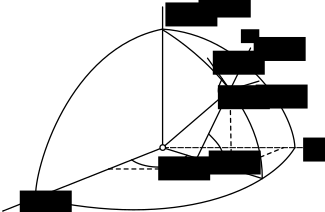
\includegraphics{./imgs/sistemas.png}
  \caption{Relación entre los sistemas local y esférico}
  \scriptsize Redibujado de Moritz y Hoffman
\end{marginfigure}



\newthought{Una parametrización} de nuestro modelo esférico nos permitirá trabajar directamente sobre
la superficie de la esfera con comodidad, y va además en consonancia con el enunciado de nuestro problema,
que dice expresamente que trabajaremos con datos accecibles desde la superficie, y para determinar
posiciones con presicion sobre la misma.

La parametrización que surge de considerar las coordenadas esféricas \(M(r=k,\varphi,\upphi)\) sería
suficiente para nuestros propósitos. Sin embargo, utilizaremos una versión modificada de la misma,
\(M(r=k,\lambda,\varphi)\), donde utilizamos la latitud \(\varphi\) se mide con respecto al
plano \(xy\), en lugar de la colatitud \(\upphi\), que se mide con respecto al eje \(Z\).

\begin{marginfigure}
  \label{fig:esfericas}
  a)
  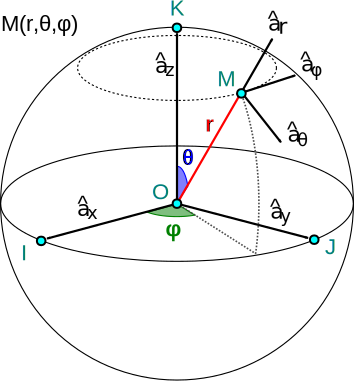
\includegraphics{./imgs/colatlon.png}
  b)
  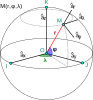
\includegraphics{./imgs/latlon.png}
  \caption{Sistema de coordenadas esféricas tradicional y coordenadas geográficas \(\varphi,\lambda\)}
  \scriptsize  CC BY-SA 3.0, Reelaborado a partir de el trabajo https://commons.wikimedia.org/w/index.php?curid=5624712

\end{marginfigure}
 

\newthought{Los problemas geodésicos} surgen a partir de la necesidad de vincular los sistemas que
llamamos locales en dos puntos diferentes de nuestra tierra-esfera. Normalmente se los denomina
como problema directo y problema inverso.

El problema geodésico directo consiste en hallar las coordenadas \(\varphi_1,\lambda_1\) de un punto
de destino a partir de las coordenadas de un punto de origen, el azimut de la dirección desde el
punto origen al de destino, y la distancia medida entre ambos \(\varphi_0, \lambda_0, \alpha_{01}, d_{01} \).
Nótese que para realizar la medición de \(\varphi_0, \alpha_{01} y d_{01}\) basta con utilizar
el sistema local origen, donde estas tres cantidades están perfectamente definidas.

El problema geodésico inverso consiste en, dadas las coordenadas \(\varphi_o,\lambda_o,\varphi_1,\lambda_1\)
de dos puntos cualesquiera, hallar la distancia entre ambos y los acimut correspondientes,
\(d_{01},\alpha_{01},\alpha_{10}\).

Sobre la solución de estos problemas baste decir que existe y que no implica ningun supuesto adicional
a los que ya se hicieron. Vale si aclarar, que el radio terrestre \(r=k\) entra como un parámetro
dentro de la solución de ambos problemas.

\newthought{Para determinar nuestro modelo de tierra} nos faltará en consecuencia hallar un valor para
el radio. Esto puede realizarse fácilmente si se parte de puntos con \(\varphi_o,\lambda_o,
\varphi_1,\lambda_1\) conocidas, y se mide \(d_{01},\alpha_{01},\alpha_{10}\). La única dificultad
de este planteo está en que la coordenada \(\lambda\) depende de la pocicion del eje X de nuestro modelo,
que había quedado indeterminada, y además esta coordenada no es accesible desde los sistemas locales
\(xyz\).

Ambas dificultades son salvables. Para uno de los puntos es posible definir el eje \(X\) en forma arbitraria
de modo que \(\lambda=0\). Luego, con esta orientación ya definida, podemos tomar el otro punto sobre
el mismo plano meridiano, haciendo uso del azimut astronómico para garantizar esta condición. De este modo,
tenemos acceso a todos los datos necesarios para calcular el radio terrestre.

\subsection{Validando nuestro primer modelo}

Utilizando las definiciones y mediciones realizadas, un observador podría realizar cálculos a partir de
los problemas geodésicos, para construir una poligonal cerrada sobre la tierra, verificando si el error
obtenido al regresar al punto de origen es compatible con la precisión de los intrumentos.

\begin{marginfigure}
  \label{fig:poligonalgeodesica}
  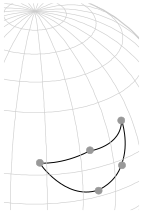
\includegraphics{./imgs/geopoly.png}
  \caption{Una poligonal geodésica como la que se plantea para validar el modelo adoptado.}
\end{marginfigure}

Otra experiencia que podría realizarse es la de utilizar la metodología descripta anteriormente para el
cálculo del radio terrestre, aplicandola a distintos pares de puntos, ubicados a distintas latitudes.

Cualquiera de estas metodologías nos llevará al hallazgo de que el modelo esférico no se ajusta
perfectamente a la tierra. En el primer caso obtendremos un error de cierre mayor al que correspondería
con el instrumental utilizado, mientras que en el segundo de los casos observaremos que la estimación
del radio terrestre varía con la latitud.

Del análisis de estas mediciónes, y a partir de la consideración de la influencia de la rotación terrestre
sobre la distribución de su masa y sobre su propio campo gravitatorio, a la luz de las teorías desarrolladas
por Isaac Newton, descubriremos que existe un modelo geométrico más apropiado que el que elegimos.
Este modelo es el de el elipsoide de revolución.

\subsection{El modelo elipsoidico de la tierra}

\newthought{El elipsoide es una superficie} cuádricas, definida por la ecuación de forma canónica:

\begin{equation*}
\frac{x^2}{a_1^2}+\frac{y^2}{a_2^2}+\frac{z^2}{b^2}=1
\end{equation*}

\begin{marginfigure}
  \label{fig:sistemas}
  a)
  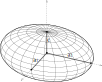
\includegraphics{./imgs/triaxial.png}
  b)
  \includegraphics{./imgs/elipsoide.png}
  \caption{Elipsoide triaxial y de revolución.}
  \scriptsize CC BY-SA 4.0, Reelaborado a partir del trabajo en https://commons.wikimedia.org/w/index.php?curid=45585493
\end{marginfigure}
 
\newthought{El elipsoide de revolución} es en particular caso en que \(a_1=a_2\),
siendo éste conocido con el nombre de elipsoide de revolución, llamado así porque
surge de hacer girar la elipse de ecuación

\begin{equation*}
{\frac{x^{{2}}}{a^{{2}}}+\frac{z^{{2}}}{b^{{2}}}=1}
\end{equation*}

perteneciente al plano \(XZ\), alrededor del eje \(Z\), coincidente con el eje menor
de la elipse. 
 
Los ejes \(a\) y \(b\) bastan para definir a la elipse y al elipsoide de revolución
correspondiente. Sin embargo no es poco comun definir al elipsoide con respecto a
parámetros cuya definicion en este momento no es procedente.

\newthought{ Para trabajar sobre el elipsoide} basta con definir la latitud en base a la
linea perpendicular al mismo, a la que podemos llamar vertical elipsoidal, y definir la
longitud y el azimut en forma análoga a como lo hicimos en la esfera.

Bastan estas definiciones para resolver en forma teórica los problemas geodésicos,
dentro de los cuales ingresaran como incognita las longitudes de los ejes \(a,b\) en
lugar de un único radio.

Siguiendo la metodología antes planteada, se pueden realizar mediciones a partir de
los sistemas locales al igual que describimos para la esfera, y a partir de las ecuaciones
de los problemas geodésicos resolver un problema de optimización para hallar los valores
de \(a\) y \(b\) que mejor se ajusten a la evidencia empírica.

Estos cálculos fueron realizados en numerosas oportunidades a lo largo de la historia
de la geodesia, desde al el siglo XVIII en adelante. Los resultados obtenidos, si bien
fueron mejorando en presicion a lo largo del tiempo, siempre llevaron a la conclusión
de que el modelo elipsoidal es suficiente para realizar los calculos que son necesarios
para ajustar las mediciones realizadas desde distintos puntos de la superficie, es decir
para vincular los sistemas locales planteados. En suma, la solución de los problemas
geodésicos en el caso elipsoidal demostró ser suficientemenete precisa como para
resolver el problema del datum.

\subsection{La Materialización del DATUM}

Hasta ahora, mencionamos que asociamos al elipsoide o a la esfera una terna cartesiana \(XYZ\)
y asumimos que el origen de esta terna debia ser coincidente con el centro de la tierra.
No entraremos en discuciones sobre cual es el centro de la tierra sino que asimilaremos este
concepto al de centro de masas.

\newthought{Para todas las mediciones} y experimentos que planteamos, partimos de nuestros
sistemas locales, obtuvimos las cantidades necesarias por observación, ya sea latitudes,
azimut, direcciones o distancias, y realizamos cálculos suponiendo que esto implicaba a los
supuestos del parrafo anterior. Sin embargo, es fácil ver que esto no es así.

En caso de que realmente la utilización de latitudes astronómicas en fuera absolutamente
compatible con el uso de latitudes elipsoidales provenientes de la solución del problema
geodésico directo, quedaría demostrada la coincidencia de las verticales astronómicas y
elipsoidales en todos los puntos. Esto implicaria a su vez que las superficies equipotenciales
terrestres son efectivamente elipsoides de revolución lo cual no es cierto.

Por este motivo, al resolver el problema geodésico directo partiendo de una observación
astronómica, la latitud de destino obtenida no coincidirá exactamente con la latitud astronómica
medida en el lugar de destino. Sin embargo, está amplicamente demostrado en la teoría y
sobre todo en el uso, que el modelo elipsoidal es suficiente como marco de referencia para
resolver el problema del datum tal como lo planteamos. Solo Resta analizar cual es la posicion
del elipsoide y de su terna de referencia \(XYZ\) con respecto al centro y eje de rotación de la
tierra real.

\newthought{ La ubicación de la terna XYZ con respecto a la tierra} queda definida forzosamente al
comenzar una medición geodésica con una observación astronómica. Esta metodología supone que en
el lugar de inicio de la medición la vertical del lugar coincide con la vertical del elipsoide, y
que el azimut al norte es el mismo en sentido astronómico que sobre el elipsoide. De esta manera,
el punto de arranque de las mediciones se convierte en lo que comunmente se llama \textbf{punto datum}.

Queda en evidencia así, la utilidad de determinar coordenadas elipsoidicas para determinados puntos
de manera que al iniciar una nueva medición podamos utilizar estas en lugar de las astronómicas,
de modo que trabajemos siempre utilizando los mismos supuestos de origen y orientación de los ejes
\(XYZ\) de referencia del elipsoide. A esta tarea se le denomina materializacion de un datum o
materialización de un \textbf{sistema de referencia} \footnote{}. Al producto de esta operación se le denomina
\textbf{marco de referencia}\footnote{}.

\newthought{ La arbitrariedad en la elección de un unico punto datum} nos lleva a considerar la construcción
de convenciones mas complejas a la hora de materializar un sistema de referencia. Para evitar un sesgo
injustificado seria razonable, por ejemplo, realizar determinaciones astronómicas sobre puntos distribuidos a lo
largo de un area de interés, agregar a ellas mediciones geodésicas de direcciones y distancias, y luego incluir
toda esta información en un problema de optimización donde se dejan libres los parametros que representan
la ubicación y orientación del elipsoide, o lo que es lo mismo, de sus ejes asociados \(XYZ\).

\begin{marginfigure}
  \label{fig:puntodatum}
  \includegraphics{./imgs/puntodatum.jpg}
  \includegraphics{./imgs/dospuntosdatum.jpg}
  \caption{ubicación del elipsoide con un único punto datum o utilizando dos puntos datum y dejando libres
  los parámetros del elipsoide.}
\end{marginfigure}

Dos casos particulares de esta metodología que vale la pena considerar son los siguientes. Existe la posibilidad de,
si el area de medición es suficientemente grande, suponer que la inclución de los radios del elipsoide \(a\) y \(b\)
como parámetros a optimizar mejore el resultado final. Esto se ha realizado en numerosas ocaciones, dando origen a
distintos parámetros de elipsoide que son utilizados al trabajar en distintos datum. Una consecuencia poco conveniente
de esta situación es que en muchas oportunidades se asocia en forma incorrecta el concepto de \textbf{datum} al conjunto
de los parámetros que definen la geometría del elipsoide, ignorando el problema de la ubicacion del mismo con respecto
a la tierra. Esta metodología, y la de selección de un único \textbf{punto datum} nos lleva a la realizacion de lo que
conocemos como \textbf{datum local}. Un ejemplo familiar para nosotros es el datum Campo Inchauspe '69

Otro caso, que es mas beneficioso de considerar, es aquel en el que se dispone de mediciones homogeneamente
distribuidas en la superficie de toda la tierra.
En este caso, es razonable suponer que la optimizacion de los parámetros nos llevará a una ubicación de la terna de
referencia donde el origen coincida realmente con el centro de masas de la tierra y el eje Z sea colineal al eje de
rotación terrestre. Este concepto es aplicado en la construcción de lo que conocemos como \textbf{datum global}

\newthought{Esta claro que la medición de la superficie completa de la tierra} es una tarea injustificada
e inpracticable para un observador o grupo de observadores que prevén tienen la necesidad de realizar mediciones
fuera de un area acotada. Este es el principal motivo de que, para permitir el desarrollo de la cartografía,
grán cantidad de paises hayan definido datum locales nacionales. Sin embargo, el avance realizado en 1957 con
la puesta en órbita exitosa del satélite \textbf{\textit{Sputnik 1}}, abrió la posibilidad de construcción de un
datum global con métodos mas simples de implementar que una campaña geodésica global.

\newthought{Dentro del marco de la física clásica}, la teoría de Newton permitió determinar como se comporta un cuerpo
que orbita a otro impulsado por la fuerza de gravedad. Las observaciones realizadas por Kepler demostraron gran presición
en la predicción de las órbitas de los cuerpos celestes. Partiendo de estas ideas, podemos suponer que la medición de
la orbita de un satélite a partir de estaciones fijas en tierra nos permitirá determinar la posición del centro de masas
terrestre con respecto a estas estaciónes.

\newthought{Con la introducción de los efectos relativistas} en la física, el cálculo de las órbitas se volvió aún más
preciso, aunque queda fuera de nuestro alcance el explicar los detalles. Baste decir que, lo unico que restaba para la
materialización de un datum ``espacial'', era el desarrollo de un metodo adecuado de medición de la distancia entre
las estaciones en tierra y el satélite en su órbita.

No demoró mucho tiempo la creación de métodos adecuados. Dos días después del lanzamiento del \textbf{\textit{Sputnik}},
se comenzó a idear un sistema que aprovechara el efecto doppler de las ondas de radio emitidas por el satélite
para la medición de la necesitada distancia. En 1959 se
intentó el primer lanzamiento de un satelite dedicado a este tipo de mediciónes por parte de los Estados Unidos,
aunque el primer lanzamiento exitoso ocurrió en 1960, considerandose el sistema, conocido como \textbf{Transit} como
completamente funcional a partir de 1967. La USSR lanzó su propio sistema de este tipo, comenzando en 1967, llamado
sucesivamente a sus versiones \textbf{Tsiklon}, \textbf{Tsikada} y \textbf{Parus}.
Sin embargo, durante el período de desarrollo de este sistema, otros sistemas se idearon y llevaron a la práctica.
Por ejemplo, el sistema SLR (\textit{Satellite Laser Ranging}), sistema de medición con laser a satélites en órbita
fue llevado a la práctica con éxito en 1964 por la NASA estadounidense.
Cabe mencionar el uso de Interferometria con Radiotelsecopios (VLBI), cuyas aplicaciones geodésicas también comenzaron
a ser aprovechadas a partir de los años 70, determinando con mucha precición la orientación de vectores sobre
la superficie terrestre. A modo aclaratorio, hacemos notar que el sistema SLR tiene muy buena precicion en la
determinación del geocentro, al basarse en la medición de órbitas cercanas a la tierra, y el sistema VLBI tiene
muy alta presición en la determinación de la orientación del eje de rotación terrestre, al referirse a fuentes
naturales de ondas de radio extremádamente lejanas a la tierra.

\newthought{La materialización de un datum global fue entonces posible}, centrando la terna de referencia en el verdadero
centro de masas de la tierra y alineandola con su eje de rotación.

A partir de la aparicion posterior de sistemas mas complejos como GPS (Global Positioning System),
GLONASS (Global'naya Navigatsionnaya Sputnikovaya Sistema) o DORIS (Détermination d'Orbite et
Radiopositionnement Intégré par Satellite), la redundancia de datos permitió una sofisticación del
método, siendo que el sistema permite al mismo tiempo la determinación de orbitas de los satelites,
pero estos están suficientemente lejanos como para tener buena precision en las orientaciones, una
vez que se corrigen los multiples errores que se producen a lo largo del camino que recorren las ondas
de radio utilizadas en la medición.

\subsection{La materialización del datum global}

Para cerrar esta sección haremos un breve resumen de cómo se llega a la materialización de un datum
global sobre la tierra, y en que forma viene esta dada. Incluimos esto para hacer un desorrollo completo
y para que el lector se forma una idea de como se relaciona este tipo de datum con los datum locales
antes estudiados.

\newthought{Al inicio de las observaciones}, se tiene una posición teórica de las órbitas de diferentes
satélites, que no tiene en cuenta ninguna anomalia en el campo gravitarorio terrestre. Se tienen una
cantidad de puntos de observación con estaciones midiendo en las técnicas GPS, SLR, VLBI y DORIS.
En primera instancia, asumiremos que el sistema DORIS provee una información similar al sistema GPS,
dado que ambos operan en frecuencias parecidas y tendrían fuentes de error similares.

Los datos con los que contamos son básicamente mediciones de distancias desde o hacia
distintos satélites obtenidos por las técnicas GPS, DORIS y SLR, a lo largo de una cantidad
considerable de tiempo, que supondremos suficiente grande con respecto al período orbital
de los satélites como para estimar sus parámetros.

Conocemos expresiones mas o menos complicadas para la trayectoria de las órbitas,
dependiendo de las perturbaciones que consideremos significativas. Por ejemplo, podemos
considerar las perturbaciones por la inhomogeneidad en el campo gravitatorio terrestre
con mayor o menor grado de detelle, agerando o quitando parámtros al sistema.

Tenemos mediciones de distancias entre puntos en la tierra a partir de la técnica
de VLBI, orientados con mucha presición a un eje que podemos considerar inmóbil
en el espacio. La determinación de la orientación relativa entre estos vectores,
depende de la presición en la determinación de los parámetros de rotación terrestre.

Tenemos expresiones que constituyen un modelo de la rotación terrestre, que
deberá forzosamente tenerse en cuenta para considerar el movimiento relativo
entre sitios receptores y satélites.

\newthought{Sugerimos un esquema de procesamiento}, a modo de ejemplo, para pasar
de esta información a la materialización de un marco de referencia geocéntrico.

En un primer paso, utilizando las expresiones de las órbitas satelitales, el modelo
de rotación terrestre, y todas las distancias observadas, se realizará un primer
ajuste de los parámetros del sistema, obteniendo valores y ecuaciones que nos
describirán trayectoria de las orbitas, la posición de los puntos considerados sobre
la superficie terrestre, y parámetros de rotación terrestre que vinculan la posición
de las estaciones con la posición de las orbitas.

Sobre este primer modelo podemos hacer algunas consideraciones. En primer lugar,
el error en la determinación de los parámetros orbitales no está correlacionado
con una posición a-priori del centro de la tierra, dado que esto no se incluyó
como variable en el modelo. En segundo lugar, la posicion del eje de rotación
terrestre que surge de este modelo está ligado a la presicion con la que se
determinaron la órbitas y los parámetros de transformación.

En consecuencia, este primer resultado nos provee de una buena determinacion
de las órbitas satelitales, pero los parámetros que nos interesan para la
determinación del marco de la tierra pueden ser calculados con mayor presición
si se realiza un nuevo cálculo.

\newthought{ Para la determinación del geocentro}, puede realizarse un ajuste
utilizando las características de las órbitas, que por como fueron calculadas, es
decir ``atadas'' a los puntos en la superficie, nos darán una observación
independiente de la posición del geocentro con respecto a ellas. Esto debe hacerse
a partir de una interpretación física de las orbitas, y eventualmente debe
considerarse en el ajuste la inhomogeneidad del campo gravitatorio terrestre.
En este ajuste cada orbita tendrá un peso diferente dependiendo de la presición
obtenida en el calculo anterior y de los errores propios de cada metodo de
medición.

\newthought{ Para la determinación de la posición del eje de rotación} debemos
agregar a la información ya procesada la nueva posición del geocentro calculada,
considerando que el eje forzosamente pasará por el centro de masas terrestre.
En segundo lugar, pero no con menos importancia, debemos incorporar la información
que sobre la rotación nos provee la evolución de los vectores medidos por VLBI,
que al estar referidos a un eje inmobil en el espacio nos brindan una información
precisa, y lo que es más importante, independiente de la determinación de las
órbitas satelitales.

\newthought{ Incluyendo esta información} en un nuevo ajuste general del sistema
obtendremos posiciones para los puntos sobre la superficie terrestre que estarán
ahora dentro de una terna que está centrada en el centro de masas de la tierra y
orientada con su eje de rotación, con la máxima precision que permiten los medios
disponibles. Solo resta asociar a la terna un elipsoide adecuado, y el marco de
referencia queda materializado.

\newthought{ Podemos preguntarnos en que forma } se da la materialización del sistema.
La respuesta es directa, las coordenadas \(\varphi,\lambda,h\) que se determinan con
el cálculo descripto están expresadas en el marco deseado. Los puntos utilizados para
la observación constituyen entonces nuestro marco de referencia, y siempre trabajaremos
dentro de este mismo marco si asignamos a ellos las coordenadas que se obtuvieron en
este cálculo. Esta es la metodología utilizada para materializar los datum más utilizados
en la actualidad, Por ejemplo ITRF, o WGS84.

\subsection{Aclaraciones posteriores}

Resta, por motivos de completitud, mencionar que un marco de referencia determinado
de este modo queda expresado en función de un tiempo determinado. Esto no sería así
en caso de que la tierra fuera un cuerpo realmente sólido. Sin embargo la realidad
es que las masas se reditribuyen dentro de la tierra continuamente. En primera
instancia el eje de rotación terrestre no es completamente estable. Debido a varios
factores externos, existe lo que se comoce como movimiento polar, que implica que
la posicion de los polos geográficos varie con el tiempo. Además, la tectónica de
placas, que es el mecanismo por el cual el calor propio de la tierra se disipa
al espacio, está continuamente desplazando los contienentes entre si haciendo que
se alejen o se acerquen, y también produce cambios en la distribucion de masas
del interior terrestre, que afectan a la posición del geocentro y a la orientación
del eje de rotación.

\newthought{Si consideramos estos efectos en la materialización del marco}, veremos
que podemos incluir el cálculo la deriva polar y la deriva continental agregando
parámetros a ajustar y aprovechando la orientación absoluta que nos provee el
método VLBI. A pesar de esto, debemos definir para que tiempo es valido el marco,
ya que si las coordenadas, es decir la materialización, varia continuamente, es
necesario saber el momento exacto para el cual las posiciones dadas fueron válidas.
Esto nos introduce al concepto de época de un marco de referencia, que está fuera
de nuestra intención explicar. Solo aclararemos que, conocida la epoca de un marco
y las trayectorias estimadas de los puntos que lo materializan, puede realizarse
la transformación entre una medición realizada en epoca actual y la epoca de referencia
del marco, en caso de que se necesite trabajar a ese nivel de detalle.

\newthought{ Sin ir en desmedro de esto}, y considerando que las placas tectónicas pueden
tratarse como bloques cuasi-estables, no es perjudicial a grán cantidad de trabajos
topográficos y geodésicos realizar los cálculos directamente en la época de referencia,
especialmente si podemos asumir con fundamento que la deformacion neta del area de trabajo
no es significativa en el tiempo.

\newthought{ Aclaramos, como nota final a esta sección}, que una vez materializado un
marco de referencia, se puede realizar una densificación con el método que sigue. Primero
se computan los parámetros de las órbitas satelitales GPS o GLONASS con respecto a los puntos incluidos
en la materialización original del marco, luego se calculan las posiciones de una cantidad
de puntos mayor, que incluya algunos de los puntos originales, a partir de estas órbitas.
Finalmente, se ajusta la posicion de los puntos comunes entre la densificación y el marco
origen, de modo que coincidan en el tiempo. Este último paso ayuda a absorver errores que
pueden haber quedado ocultos dentro de los parámetros originalmente estimados en el marco,
de modo que el marco y la densificación sean realmente compatibles. Ésta es la forma
en que está construido el marco POSGAR07, Marco de referencia oficial de la republica argentina,
que consituye una densificación del marco global ITRF08.

\section{\(2+1\neq3\) Los Datum Altimétricos }

\newthought{Hasta ahora hemos considerado un datum planimétrico}. Las coordenadas que obtuvimos
dentro de nuestros marcos de referencia locales eran sólo \(\varphi,\lambda\), determinando un
punto sobre la superficie del elipsoide. Cuando hablamos de datum global mencionamos las coordenadas
\(\varphi,\lambda,h\), aunque no introdujimos de que hablabamos al mencionar ``h''.

\newthought{La altura elipsoidal \(h\)} queda definida como la distancia de un punto al elipsoide
de referencia del datum medida sobre la perpendicular al mismo. En este sentido, el datum global
que propusimos es un datum tridimensional, porque, al no trabajar con coordenadas elipsoidales
hasta el final del desarrollo, utilizamos las posiciones tridimensionales de los puntos, quedando
implícita la coordenada h además de \(\varphi,\lambda\).

\newthought{La altura sobre el nivel del mar}, es la forma en la que se trabaja con la altura
al utilizar datums geodésicos locales. Al definir el datum horizontal a partir de mediciones
astronómicas, se trabaja en todos los puntos con altura \(h=0\), y se define un criterio
separado para la medición de alturas.

Considerando que, como ya vimos, las superficies equipotenciales terrestre no
son superficies elipsoidales. Una medición de altura que sea independiente de la determinación
de la posición, por ejemplo basada en la utilización de planos horizontales, como la nivelación
geométrica, diferirá de la altura elipsoidal. La aplicación de correcciónes a esta altura
a partir de mediciones de gravedad garantizará la coherencia del sistema, pero no
permitirá asociar la altura a la altura elipsoidal.

Esto es un problema cuando trabajamos con datos provenientes de distintos sistemas. Sin embargo,
un modelado de la superficie equipotencial terrestre de altura 0, normalmente llamada \(W_0\) o
geoide, que esté referida a posiciones elipsoidales en un datum global conocido
puede resolver la dificultad. La calidad de esta solucion dependerá de la rugosidad del
geoide real en la zona y de la definición y presición con que esté calculado el modelo
de geoide. Mencionamos algunos ejemplos de modelo de geoide como referencia. Dos ejemplo modernos
que podemos mencionar son EGM08 y EIGEN-6C4.

\section{Transformaciones de datum}

\newthought{Partiendo de la metodología de construcción} de un datum, y habiendo definido
que significa que un dato esté provisto en distintos datum, dedicaremos esta sección
a evaluar que implica contar con información provista en diferentes datum, y a presentar
metodologías que nos permitan compatibilizar esta información.





%\section{El Elipsoide}
%
%\ \ La geometría del elipsoide es más complicada que la de la
%esfera, por lo que se hace necesario detallar algunos conceptos al
%respecto.
%
%\subsection*{Parámetros del elipsoide}
%
%El elipsoide  de revolución, utilizado en geodesia viene definido en su forma canónica
%por la ecuación
%
%\begin{equation*}
%\frac{x^2}{a^2}+\frac{y^2}{a^2}+\frac{z^2}{b^2}=1
%\end{equation*}
%
%donde \(a\) se conoce como semieje mayor y \(b\) como semieje menor o eje de revolución. 
%
%\ \ El elipsoide se denomina de revolución, porque se obtiene haciendo
%girar la elipse:
%
%\begin{equation*}
%{\frac{x^{{2}}}{a^{{2}}}+\frac{z^{{2}}}{b^{{2}}}=1}
%\end{equation*}
%perteneciente al plano xz, alrededor del eje menor. 
%
%\ \ Los ejes \(a\) y \(b\), definen perfectamente a la elipse y al
%elipsoide de revolución correspondiente, es por esto que se los conoce con el nombre de
%parámetros del elipsoide.
%
%Sin embargo, existen otros parámetros que suelen utilizarse, y
%en algunos casos simplifican los calculos.
%
%\begin{table}
%  \center
%\begin{tabular}{cc}
%\toprule
%semieje mayor & \(a\) \\ 
%semieje menor & \(b\) \\
%
%aplastamiento &
%
%\(
%\alpha =\frac{a-b}{a}
%\) \\
%
%primera excentricidad &
%
%\(
%e^2=\frac{a^2-b^2}{a^2}
%\) \\
%
%y segunda excentricidad & 
%
%\(
%e'^2=\frac{a^2-b^2}{b^2}
%\) \\
%\bottomrule
%\end{tabular}
%\end{table}
%
%De los cinco parámetros definidos:  \( a,b,\alpha ,\beta ,e^2,e'^2\),
%solo se necesitan dos para definir la elipse y el correspondiente
%elipsoide de revolución. Por ejemplo, los más usados son:
%
%\ \ a y b  {}-  a y e2  {}-  a y ${\alpha }$
%
%\subsection{Coordenadas Elipsóidicas}
%
%\ \ De la misma forma que se definió para la esfera, se puede concebir
%un sistema de coordenadas elipsóidicas referidas a un eje y un plano
%fundamental.
%
%\ \ Cortando el elipsoide con planos cualesquiera, las secciones son
%siempre elipses; en el caso particular de los planos paralelos al plano
%xy, es decir normales al eje z, las secciones son circunferencias de
%radio variable, llamados paralelos elipsóidicos. 
%
%\ \ Los planos que contienen al eje z, cortan al elipsoide según
%elipses iguales, llamados meridianos elipsóidicos. 
%
%\begin{marginfigure}
%\includegraphics{./imgs/repslatex-img48.png}
%\end{marginfigure}
% 
%
%\ \ El eje fundamental del sistema de referencia es el eje de
%rotación, el plano fundamental es el que es normal al eje de
%revolución y pasa por el centro del elipsoide, corta al mismo en una
%sección circular llamada ecuador elipsóidico, cuyo radio es el
%semieje mayor de la elipse {\textquotedblleft}a{\textquotedblright}.
%
%\begin{marginfigure}
%\includegraphics{./imgs/repslatex-img49.png}
%\end{marginfigure}
% 
%
%\ \ Dado un punto P cualquiera sobre el elipsoide, es posible trazar un
%plano tangente a la superficie que contenga a P, la recta que pasa por
%P y es perpendicular al plano tangente, se denomina
%{\textquotedblleft}normal al elipsoide{\textquotedblright}.
%
%\ \ La latitud elipsóidica  ${\varphi }$ o geodésica del punto P
%sobre el elipsoide se define como el ángulo entre la normal en P y el
%ecuador elipsóidico; se mide de 0 a 90{\textordmasculine}, positivo
%al Norte y negativo al Sur.
%
%\ \ La longitud elipsóidica  ${\lambda }$ o geodésica del punto P es
%el ángulo diedro entre el meridiano que pasa por P y otro definido
%como origen; se mide de 0 a 180{\textordmasculine}, positivo hacia el
%este y negativo hacia el Oeste.
%
%\ \ El acimut elipsóidico A es el ángulo entre dos planos, ambos
%contienen a la normal al elipsoide en P: uno contiene a los polos y el
%otro a la dirección considerada.
%
%VIII.3.- CORTES NORMALES.
%
%\begin{marginfigure}
%\includegraphics{./imgs/repslatex-img50.png}
%\end{marginfigure}
% 
%
%\ \ Dada una superficie cualquiera, se puede considerar en un punto P
%sobre la misma un haz de infinitos planos que contienen a la normal a
%la superficie en P. Dichos planos son llamados planos normales y
%determinan \textbf{secciones normales}.
%Las secciones normales al elipsoide son las que se obtienen de la
%intersección de la superficie con los planos que contienen la normal
%al elipsoide. Existen infinitas secciones normales en todo punto P del
%elipsoide; todas son elipses en el caso del elipsoide de revolución.
%Las secciones se caracterizan por acimut. Así habrá una sección
%de acimut cero: llamada de sección meridiana, y otra de acimut de
%90°: la sección normal al meridiano.
%
%\subsection{Radios de Curvatura}
%
%\ \ Los radios de curvatura que son de interés son los de las
%secciones normales al elipsoide, y si existen infinitas secciones
%normales hay infinitos radios de curvatura.
%
%\begin{marginfigure}
%\includegraphics{./imgs/repslatex-img51.png}
%\end{marginfigure}
% 
%
%\ \ Dada una curva plana se define como curvatura media, al cociente
%entre el ángulo que forman las tangentes a la curva en los puntos
%extremos del arco y la longitud del arco; por lo tanto:
%
%\begin{equation*}
%{C_{{m}}=\frac{\mathit{\Delta \varphi }}{\mathit{\Delta S}}}
%\end{equation*}
%
%\begin{equation*}
%\Delta S >> AB
%\end{equation*}
%
%Se llama curvatura en un punto A, al límite:
%
%\begin{equation*}
%  C = \lim_{\Delta S \to 0} \frac{\Delta \Phi}{\Delta S} = \frac{d \Phi}{dS}
%\end{equation*}
% 
%
%En una circunferencia, la curvatura será:
%
%\begin{equation*}
%{\frac{\mathit{d\varphi
%}}{\normalsubformula{\text{dS}}}=\frac{\mathit{d\varphi }}{R\cdot
%\mathit{d\varphi }}}
%\end{equation*}
%\begin{equation*}
%{C=\frac{1}{R}}
%\end{equation*}
%La curvatura es la inversa del radio. Se llama en general radio de
%curvatura en un punto de una curva dada, al valor recíproco de la
%curvatura dada en el punto; su valor está dado por:
%
%\begin{equation*}
%{R=\frac{\left(1+y'^{{2}}\right)^{{\frac{3}{2}}}}{y\text{{\textquotesingle}{\textquotesingle}}}=\frac{\left(1+\left(\frac{\normalsubformula{\text{dy}}}{\normalsubformula{\text{dx}}}\right)^{{2}}\right)^{{\frac{3}{2}}}}{\frac{d^{{2}}y}{\normalsubformula{\text{dx}}^{{2}}}}}
%\end{equation*}
%
%De los infinitos radios de curvatura de las secciones normales en un
%punto del elipsoide, habrá uno de valor máximo y otro de valor
%mínimo, llamados radios principales de curvatura, y son:
%
%\ \ M: el radio de curvatura del meridiano o sección meridiana.
%Corresponde a acimut cero, y es el menor.
%
%\ \ N: el radio de curvatura de la sección normal al meridiano o
%primer vertical. Corresponde a acimut de noventa grados y es el radio
%mayor.
%
%\begin{marginfigure}
%\includegraphics{./imgs/repslatex-img54.png}
%\end{marginfigure}
% 
%
%\ \ Estos radios de curvatura tienen un papel importante no solo en la
%Geodesia,  sino además en la Cartografía, en las deducciones de las
%expresiones de la proyección Gauss-Kruger, por lo tanto el
%propósito es determinar los valores de M y N en función del
%elipsoide, es decir se sus parámetros y de la posición del punto
%sobre el mismo, es decir de sus coordenadas. 
%
%\ \ Tanto M y N son función de los parámetros del elipsoide y de la
%latitud solamente, ya que sus secciones meridianas son iguales.
%
%\begin{marginfigure}
%\includegraphics{./imgs/repslatex-img55.png}
%\end{marginfigure}
% 
%
%\ \ Se parte de la ecuación de la elipse meridiana y la del radio de
%curvatura. En la elipse meridiana (Fig. VIII.7),
%{\textquotedblleft}a{\textquotedblright} es el radio del ecuador y
%{\textquotedblleft}b{\textquotedblright} el radio polar. Sea P un punto
%cualquiera sobre la elipse meridiana, el ángulo que forma la normal
%en P con el eje mayor es la latitud  ${\varphi }$. Trazando la tangente
%en el punto P, ésta forma con el eje de las x el ángulo
%(90{\textordmasculine}+ ${\varphi }$). Tanto x e y pueden considerarse
%como funciones de una única variable  ${\varphi }$, que es la que
%interesa en Geodesia y Cartografía. Se puede imaginar el punto P
%moviéndose sobre la elipse desde el ecuador hasta el polo; la latitud
%varía de 0 a 90{\textordmasculine}, x disminuye de
%{\textquotedblleft}a{\textquotedblright} a cero, e y crece de cero a
%{\textquotedblleft}b{\textquotedblright}. Si x e y son funciones de la
%latitud, también lo son sus derivadas, las que expresadas en
%función de la latitud se introducen en la ecuación del radio de
%curvatura para encontrar M y N.
%
%\ \ El radio de curvatura de la sección meridiana M es:
%
%\begin{equation*}
%{M=\frac{a^{{2}}\cdot b^{{2}}}{\left[a^{{2}}\cdot \text{cos}^{{2}}\left(\varphi \right)+b^{{2}}\cdot \normalsubformula{\text{sen}}^{{2}}\left(\varphi \right)\right]^{{\frac{3}{2}}}}}
%\end{equation*}
%
%se puede expresar también en función de la excentricidad:
%
%\begin{equation*}
%{M=\frac{a^{{2}}\cdot \left(1-e^{{2}}\right)}{\left[1-e^{{2}}\cdot \normalsubformula{\text{sen}}^{{2}}\left(\varphi \right)\right]^{{\frac{3}{2}}}}}
%\end{equation*}
%
%\ \ Para calcular el radio de curvatura de la sección normal al
%meridiano, se establece la ecuación de la elipse correspondiente a
%esa sección y se determina el radio de curvatura en el punto que
%interesa, llegando a las siguientes expresiones:
%
%\begin{equation*}
%{N=\frac{a}{\left[1-e^{{2}}\cdot \normalsubformula{\text{sen}}^{{2}}\left(\varphi \right)\right]^{{\frac{1}{2}}}}}
%\end{equation*}
%
%\begin{equation*}
%{N=\frac{a^{{2}}}{\left[a^{{2}}\cdot \text{cos}^{{2}}\left(\varphi \right)+b^{{2}}\cdot \normalsubformula{\text{sen}}^{{2}}\left(\varphi \right)\right]^{{\frac{1}{2}}}}}
%\end{equation*}
%
%\ \ Se demuestra además que el radio de un paralelo cualquiera de
%latitud  ${\varphi }$; ver fig VIII.7:
%
%\begin{equation*}
%{r=N\cdot \text{cos}\left(\varphi \right)}
%\end{equation*}
%Por lo tanto:
%
%\begin{equation*}
%{N=\frac{r}{\text{cos}\left(\varphi \right)}}
%\end{equation*}
%de donde N es el segmento PK de la Figura VIII.7.
%
%\ \ Para algunas deducciones puede ser necesario que los radios de
%curvatura se expresen en función de la segunda excentricidad; se
%determina que:
%
%\begin{equation*}
%{M=\frac{a^{{2}}}{b\cdot \left[1+e'^{{2}}\cdot \text{cos}^{{2}}\left(\varphi \right)\right]^{{\frac{3}{2}}}}}
%\end{equation*}
%
%\begin{equation*}
%{N=\frac{a^{{2}}}{b\cdot \left[1+e'^{{2}}\cdot \text{cos}^{{2}}\left(\varphi \right)\right]^{{\frac{1}{2}}}}}
%\end{equation*}
%
%Los valores en el polo se encuentran haciéndolo  ${\varphi =\text{90}}$ y se obtiene:
%
%\begin{equation*}
%{M=N=\frac{a^{{2}}}{b}}
%\end{equation*}
%En el ecuador  ${\varphi =0}$, se tiene que:
%
%\begin{equation*}
%{M=a\cdot \left(1-e^{{2}}\right)}
%\end{equation*}
%\begin{equation*}
%{N=a}
%\end{equation*}
%donde M es menor que N; se evidencia que N es siempre mayor que M,
%llegándose a igualar en el polo.
%
%\ \ Se deduce también que el radio de curvatura de una sección
%normal de acimut cualquiera es igual a:
%
%\begin{equation*}
%{R_{{A}}=\frac{M\cdot N}{M\cdot \normalsubformula{\text{sen}}^{{2}}\left(A\right)+N\cdot \text{cos}^{{2}}\left(A\right)}}
%\end{equation*}
%
%\ \ En muchas aplicaciones geodésicas y cartográficas, es
%suficientemente aproximado utilizar una esfera auxiliar que reemplaza
%al elipsoide, cuya superficie se adapta lo mejor posible en las
%proximidades del punto de interés.
%
%\ \ Esta esfera tiene un radio, que es el valor medio de todos los
%radios de curvatura del elipsoide en un punto; esto es:
%
%\begin{equation*}
%{R=\frac{1}{\left(\wideslash{\pi }{2}\right)}\cdot \overset{{A=\wideslash{\pi }{2}}}{\underset{{A=0}}{\int }}{R_{{A}}\cdot \normalsubformula{\text{dA}}}}
%\end{equation*}
%Se demuestra que el radio de la esfera que mejor se adapta es:
%
%\begin{equation*}
%{R=\sqrt{M\cdot N}}
%\end{equation*}
%
%VIII.5.- ARCO DE MERIDIANO ELIPSÓIDICO.
%
%\begin{marginfigure}
%\includegraphics{./imgs/repslatex-img56.png}
%\end{marginfigure}
% 
%
%\ \ Si se desea calcular la longitud la longitud de un arco de meridiano
%entre dos puntos P1 y P2, teniendo en cuenta que un diferencial de arco
%está dado por:
%
%\begin{equation*}
%{\normalsubformula{\text{dS}}=M\cdot \mathit{d\varphi }}
%\end{equation*}
%Se debe integrar dicho elemento entre los valores de  ${\varphi _{{1}}}$
%y  ${\varphi _{{2}}}$; esto es:
%
%\begin{equation*}
%{S=\overset{\varphi _{{2}}}{\underset{{\varphi _{{1}}}}{\int }}{M\cdot
%\mathit{d\varphi }}}
%\end{equation*}
%
%\begin{equation*}
%{S=\overset{\varphi _{{2}}}{\underset{{\varphi _{{1}}}}{\int}}{\frac{a\cdot \left(1-e^{{2}}\right)}{\left[1-e^{{2}}\cdot \normalsubformula{\text{sen}}^{{2}}\left(\varphi \right)\right]^{{\frac{3}{2}}}}\cdot \mathit{d\varphi }}}
%\end{equation*}
%
%\begin{equation*}
%{S=a\cdot \left(1-e^{{2}}\right)\cdot \overset{\varphi _{{2}}}{\underset{{\varphi _{{1}}}}{\int }}{\frac{\mathit{d\varphi}}{\left[1-e^{{2}}\cdot \normalsubformula{\text{sen}}^{{2}}\left(\varphi \right)\right]^{{\frac{3}{2}}}}}}
%\end{equation*}
%
%Esta integral se resuelve mediante el desarrollo de la serie binomial
%del integrando:
%
%\begin{equation*}
%\begin{matrix}{\left[1-e^{{2}}\cdot \normalsubformula{\text{sen}}^{{2}}\left(\varphi \right)\right]^{{-{\frac{3}{2}}}}=1+\frac{3}{2}\cdot e^{{2}}\cdot \normalsubformula{\text{sen}}^{{2}}\left(\varphi \right)+\frac{3}{2}\cdot {\frac{5}{4}}\cdot e^{{4}}\cdot \normalsubformula{\text{sen}}^{{4}}\left(\varphi \right)+\frac{3}{2}\cdot {\frac{5}{4}}\cdot {\frac{7}{6}}\cdot e^{{6}}\cdot \normalsubformula{\text{sen}}^{{6}}\left(\varphi \right)}\hfill\null \\+{\frac{3}{2}}\cdot {\frac{5}{4}}\cdot {\frac{7}{6}}\cdot {\frac{9}{8}}\text{.}\text{.}\text{.}\text{.}\text{.}\text{.}\text{.}\text{.}\text{.}\text{.}\text{.}\text{.}\text{.}\text{.}\text{.}\text{.}\text{.}\text{.}\text{.}\hfill\null \end{matrix}\hfill 
%\end{equation*}
%
%la cual se debe multiplicar por  ${\mathit{d\varphi }}$ y ejecutar la
%integración término por término, pero antes de proceder a la
%interpretación, se reemplazan las potencias del seno de la latitud en
%funciones trigonométricas múltiplos de  ${\varphi }$, como se
%indica a continuación:
%
%\begin{equation*}
%{\normalsubformula{\text{sen}}^{{2}}\left(\varphi
%\right)=\frac{1}{2}-\frac{1}{2}\cdot \text{cos}^{{2}}\left(\varphi
%\right)}
%\end{equation*}
%\begin{equation*}
%{\normalsubformula{\text{sen}}^{{4}}\left(\varphi
%\right)=\frac{3}{8}-\frac{1}{2}\cdot \text{cos}^{{2}}\left(\varphi
%\right)+\frac{1}{8}\cdot \text{cos}^{{4}}\left(\varphi \right)}
%\end{equation*}
%\begin{equation*}
%{\normalsubformula{\text{sen}}^{{6}}\left(\varphi
%\right)=\frac{5}{\text{16}}-\frac{\text{15}}{\text{32}}\cdot
%\text{cos}^{{2}}\left(\varphi \right)+\frac{3}{\text{16}}\cdot
%\text{cos}^{{4}}\left(\varphi \right)-\frac{1}{\text{32}}\cdot
%\text{cos}^{{6}}\left(\varphi \right)}
%\end{equation*}
%\begin{equation*}
%{\normalsubformula{\text{sen}}^{{8}}\left(\varphi
%\right)=\frac{\text{35}}{\text{128}}-\frac{7}{\text{16}}\cdot
%\text{cos}^{{2}}\left(\varphi \right)+\frac{7}{\text{32}}\cdot
%\text{cos}^{{4}}\left(\varphi \right)-\frac{1}{\text{16}}\cdot
%\text{cos}^{{6}}\left(\varphi \right)+\frac{1}{\text{128}}\cdot
%\text{cos}^{{8}}\left(\varphi \right)}
%\end{equation*}
%Estos últimos valores se reemplazan en la (VIII.10), y quedan
%multiplicados por los factores  ${\frac{3}{2}\cdot e^{{2}}}$, 
%${\frac{3}{2}\cdot {\frac{5}{4}}\cdot e^{{4}}}$, etc. Se agrupan luego
%según los cosenos múltiplos de la latitud, y para abreviar conviene
%escribir:
%
%\begin{equation*}
%{A=1+\frac{3}{4}\cdot
%e^{{2}}+\frac{\text{45}}{\text{64}}e^{{4}}+\frac{\text{175}}{\text{256}}\cdot
%e^{{6}}+\frac{\text{11025}}{\text{16384}}\cdot
%e^{{8}}\text{.}\text{.}\text{.}\text{.}\text{.}\text{.}\text{.}\text{.}\text{.}\text{.}\text{.}\text{.}\text{.}}
%\end{equation*}
%
%\begin{equation*}
%{B=-\left[\frac{3}{4}\cdot
%e^{{2}}+\frac{\text{15}}{\text{16}}e^{{4}}+\frac{\text{525}}{\text{512}}\cdot
%e^{{6}}+\frac{\text{2205}}{\text{2048}}\cdot
%e^{{8}}+\text{.}\text{.}\text{.}\text{.}\text{.}\text{.}\text{.}\text{.}\text{.}\text{.}\text{.}\text{.}\text{.}\right]}
%\end{equation*}
%
%\begin{equation*}
%{C=\overset{}{{}}\overset{}{{}}\overset{}{{}}\overset{}{{}}\overset{}{{}}\left[\frac{\text{15}}{\text{64}}e^{{4}}+\frac{\text{105}}{\text{256}}\cdot e^{{6}}+\frac{\text{2205}}{\text{4096}}\cdot e^{{8}}+\text{.}\text{.}\text{.}\text{.}\text{.}\text{.}\text{.}\text{.}\text{.}\text{.}\text{.}\text{.}\text{.}\right]}
%\end{equation*}
%
%\begin{equation*}
%{D=\overset{}{{}}\overset{}{{}}\overset{}{{}}\overset{}{{}}\overset{}{{}}\overset{}{{}}\overset{}{{}}\overset{}{{}}\overset{}{{}}-\left[\frac{\text{35}}{\text{512}}\cdot
%e^{{6}}+\frac{\text{315}}{\text{2048}}\cdot
%e^{{8}}+\text{.}\text{.}\text{.}\text{.}\text{.}\text{.}\text{.}\text{.}\text{.}\text{.}\text{.}\text{.}\text{.}\right]}
%\end{equation*}
%
%\begin{equation*}
%{E=\overset{}{{}}\overset{}{{}}\overset{}{{}}\overset{}{{}}\overset{}{{}}\overset{}{{}}\overset{}{{}}\overset{}{{}}\overset{}{{}}\overset{}{{}}\overset{}{{}}\overset{}{{}}\overset{}{{}}\overset{}{{}}\overset{}{{}}+\left[\frac{\text{315}}{\text{16384}}\cdot
%e^{{8}}+\text{.}\text{.}\text{.}\text{.}\text{.}\text{.}\text{.}\text{.}\text{.}\text{.}\text{.}\text{.}\text{.}\right]}
%\end{equation*}
%
%Reemplazando en (VIII.10) se tiene que:
%
%\begin{equation*}
%{\left[1-e^{{2}}\cdot \normalsubformula{\text{sen}}^{{2}}\left(\varphi
%\right)\right]^{{\frac{-3}{2}}}=A+B\cdot \text{cos}\left(2\varphi
%\right)+C\cdot \text{cos}\left(4\varphi \right)+D\cdot
%\text{cos}\left(6\varphi \right)+E\cdot \text{cos}\left(8\varphi
%\right)+\text{.}\text{.}\text{.}\text{.}}
%\end{equation*}
%
%Multiplicando por  ${a\cdot \left(1-e^{{2}}\right)\cdot \mathit{d\varphi}}$,
%y teniendo en cuenta la (VIII.9), se tiene que:
%
%\begin{equation*}
%{S=a\cdot \left(1-e^{{2}}\right)\overset{\varphi
%_{{2}}}{\underset{{\varphi _{{1}}}}{\int }}{\left[A+B\cdot
%\text{cos}\left(2\varphi \right)+C\cdot \text{cos}\left(4\varphi
%\right)+D\cdot \text{cos}\left(6\varphi \right)+E\cdot
%\text{cos}\left(8\varphi
%\right)+\text{.}\text{.}\text{.}\text{.}\right]}{?\mathit{d\varphi }}}
%\end{equation*}
%
%Integrando esta última expresión se obtiene el arco de meridiano
%elipsóidico entre dos valores de latitud dados; por lo tanto:
%
%\begin{equation*}
%{S=a\cdot \left(1-e^{{2}}\right)\cdot \left(A+\frac{B}{2}\cdot
%\normalsubformula{\text{sen}}\left(2\varphi \right)+\frac{C}{4}\cdot
%\normalsubformula{\text{sen}}\left(4\varphi \right)+\frac{D}{6}\cdot
%\normalsubformula{\text{sen}}\left(6\varphi \right)+\frac{E}{8}\cdot
%\normalsubformula{\text{sen}}\left(8\varphi
%\right)+\text{.}\text{.}\text{.}\text{.}\right)|_{{\varphi
%_{{1}}}}^{\varphi _{{2}}}}
%\end{equation*}
%
%En esta expresión el valor de la latitud que acompa\~na a A se debe
%introducir en radianes.
%
%En caso que se desee introducir la latitud en grados sexagesimales, hay
%que agregar en el primer término del paréntesis el factor 
%${\frac{1}{\rho _{{o}}}}$, siendo el  ${\rho _{{o}}}$ el número de
%grados contenidos en un radián.
%
%Para simplificar aún más la última expresión, se puede escribir:
%
%\begin{equation*}
%{\alpha =a\cdot \left(1-e^{{2}}\right)\cdot A}
%\end{equation*}
%
%\begin{equation*}
%{\beta =\frac{a}{2}\cdot \left(1-e^{{2}}\right)\cdot B}
%\end{equation*}
%
%\begin{equation*}
%{\gamma =\frac{a}{4}\cdot \left(1-e^{{2}}\right)\cdot C}
%\end{equation*}
%
%\begin{equation*}
%{\delta =\frac{a}{6}\cdot \left(1-e^{{2}}\right)\cdot D}
%\end{equation*}
%
%\begin{equation*}
%{\varepsilon =\frac{a}{8}\cdot \left(1-e^{{2}}\right)\cdot E}
%\end{equation*}
%
%con lo cual la expresión del arco se transforma en:
%
%\begin{equation*}
%S=\alpha \varphi + \beta sen (2\varphi) + \gamma sen (4\phi) + \delta sen (6\varphi) + \epsilon sen (8\varphi) + ... |_{\Phi1}^{\Phi2}
%\end{equation*}
%%   (VIII.11)
%\
%\ \ Por medio de las expresiones vistas se calculan de una vez, para un
%determinado elipsoide, las constantes  ${\alpha ,\beta ,\gamma ,\delta
%,\varepsilon }$, las que dependen únicamente del semieje mayor y de
%la excentricidad de la elipse meridiana. Luego con la expresión
%(VIII.11) se puede calcular un arco de meridiano entre dos valores de
%latitud cualesquiera.
%
%\ \ En Cartografía existen dos arcos de meridiano de especial
%interés, como se verá más adelante. Éstos son el arco de
%meridiano desde el ecuador hasta un punto de latitud cualquiera y el
%arco de meridiano desde el polo sur al punto de la latitud considerada,
%valores éstos que forman parte de las expresiones de las coordenadas
%de U.T.M. y Gauss-Kruger, respectivamente. 
%
%\ \ En el primer caso, \(\varphi_1=0\) , la expresión %(VIII.11)
%se transforma en:
%
% \begin{equation*}
%S=\alpha \varphi + \beta sen (2\varphi) + \gamma sen (4\phi) + \delta sen (6\varphi) + \epsilon sen (8\varphi)
%\end{equation*}
%%   (VIII.12)
%
% En el segundo \(\varphi_1=90°=\frac{\varpi}{2}\), se tiene que la %(VIII.11)
% se transforma en:
%
% \begin{equation*}
%S=\alpha \left( \varphi + \frac{\varpi}{2} \right) + \beta sen (2\varphi) + \gamma sen (4\phi) + \delta sen (6\varphi) + \epsilon sen (8\varphi)
%\end{equation*}
%%   (VIII.13)
%
%recordando que el valor de la latitud en el primer término debe
%expresarse en radianes.
%
%\ \ Hasta la oficialización del Datum POSGAR 94 La República Argentina
%utilizó como elipsoide de referencia al elipsoide Internacional (de Hayford),
%cuyos parámetros son:
%
%\begin{center}
%\ \ Semieje mayor: \(a=6.378.388 m\)
%\ \ Aplastamiento: \(\alpha = \frac {1} {297}\)   
%\end{center}
%
%En función de estos parámetros se puede calcular el cuadrado de la
%primera excentricidad y las constantes  ${\alpha ,\beta ,\gamma ,\delta
%,\varepsilon }$.
%
%\begin{marginfigure}
%  \caption{Constantes del elipsoide internacional de Hayford}
%  \begin{align*}
%    e^2 & = 0,006722670022 \\
%    a & = 6367654,500690 \\
%    \alpha & = 111136,536655 \\
%    \beta & = -16109,034378 \\
%    \gamma & = 16,976211 \\
%    \delta & = -0,022266 \\
%    \epsilon & = 0,000032
%  \end{align*}
%\end{marginfigure}
%%   (VIII.14)
%
%\begin{center}
%\begin{minipage}{6.35cm}
%
%(para introducir $\varphi $ en radianes)
%(para introducir $\varphi $ en grados)
%
%\end{minipage}
%\end{center}
%Los valores de las constantes están expresados en metros, unidad en
%que se obtiene el arco de meridiano.
%
%VIII.6.- ARCO DE PARALELO ELIPSÓIDICO.
%
%\begin{marginfigure}
%\includegraphics{./imgs/repslatex-img64.png}
%\end{marginfigure}
% 
%
%Dado que el elipsoide es de revolución, los paralelos son
%circunferencias. Un elemento de arco de paralelo está dado por:
%
%\begin{equation*}
%dp = r \, d\lambda = N \, cos(\varphi) \, d\lambda
%\end{equation*}
% 
%
%El valor de un arco de paralelo entre las longitudes  
%\(\lambda_1\) y \(\lambda_2\) está dado por:
%
%\begin{equation*}
%  AB = N \, cos(\varphi) \, (\lambda_2-\lambda_1)
%\end{equation*}
%%   (VIII.15)
%
%VIII.7.- SISTEMAS DE REFERENCIA.
%
%\ \ Para calcular las posiciones de los puntos sobre la tierra es
%necesario elegir algún sistema de referencia. Sin las coordenadas de
%los puntos de la superficie terrestre es inconcebible la
%representación de la misma es un plano, que es tarea de la
%cartografía. Tales sistemas pueden tomar diversas formas, de las
%cuales habrá que elegir la más conveniente; entre ellos:
%
%a.- Coordenadas cartesianas: x, y, z. El eje z es paralelo al eje de
%rotación de la tierra, y el eje x puede ser paralelo a Greenwich.
%Idealmente el origen (0,0,0) debería ser el centro de masa de la
%tierra.
%
%b.- Coordenadas polares geocéntricas: r, $\theta $, $\lambda $. Son
%transformaciones de las anteriores y en general no se utilizan.
%
%c.- Coordenadas elipsóidicas: $\varphi $, $\lambda $. Sobre un
%elipsoide de referencia, donde hay una correspondencia biunívoca
%entre los puntos de la tierra y los puntos sobre la figura. La tercer
%coordenada, la cota, puede ser medida a partir del elipsoide, como
%sería natural, pero para pronósticos cartográficos, las alturas
%son medidas a partir del nivel del mar.
%
%d.- Coordenadas planas: son las que registran las posiciones de los
%puntos por medio de coordenadas rectangulares X e Y, sobre una
%representación plana del elipsoide.
%
%e.- En lugar de registrar la altura de los puntos por encima del geoide,
%es posible especificarlas por su potencial gravitacional, junto con la
%latitud y la longitud.
%
%f.- Coordenadas astronómicas: las observaciones astronómicas de
%latitud y longitud, son medidas que se refieren a la dirección de la
%gravedad en el punto de observación, la cual no coincide ni es
%paralela en general a la normal elipsóidica correspondiente al punto
%sobre el elipsoide. Estas observaciones son de gran importancia e
%interés para ciertas aplicaciones, pero las líneas astronómicas
%de igual latitud y longitud no constituyen un sistema de coordenadas
%usual. 
%
%\ \ El sistema de referencia usual en las proyecciones geodésicas es
%el elipsóidico, en el cual la posición de un punto sobre la
%superficie topográfica se describe por la latitud y longitud
%elipsóidicas y su altura respecto del geoide. Para completar este
%registro sería necesario determinar la separación del geoide y el
%elipsoide.
%
%VIII.8.- UBICACIÓN DEL ELIPSOIDE.
%
%\ \ En cuanto al concepto de la figura de la tierra, se consideran tres
%superifices:
%
%a.- La superficie topográfica, sólida, irregular, con una forma
%aproximadamente elipsoidal, con semiejes de 6378 y 6357 km.
%
%b.- El geoide, que se describe como la superficie coincidente con el
%nivel medio del mar, prolongándolo idealmente debajo de los
%continentes, es la superficie que determinaría el nivel medio del mar
%si se admite que se puede circular por peque\~nos canales por debajo de
%la superficie topográfica. Más precisamente es la superficie
%equipotencial del campo de gravedad de la tierra, la cual coincide con
%el nivel medio del mar en equilibrio. El geoide es una realidad
%física, el eje vertical del teodolito es normal al geoide y el
%proceso de nivelación geométrica mide las alturas sobre el mismo.
%
%c.- El elipsoide de referencia es la figura matemática,
%geométricamente definida, sobre la cual se expresan las posiciones de
%puntos sobre la tierra, y sus ejes se aproximan al geoide lo más
%estrechamente posible. Sus meridianos y paralelos constituyen un
%sistema de referencia.
%
%\ \ La definición de un sistema elipsoidal implica la elección de
%los ejes mayor y menor del elipsoide, o el eje mayor y el
%aplastamiento. Se han utilizado muchos valores diferentes, y se han
%acordado valores internaciones, pero la mayoría de los países
%continúan usando otros elipsoides.
%
%\begin{marginfigure}
%\includegraphics{./imgs/repslatex-img69.png}
%\end{marginfigure}
% 
%
%\ \ Otro aspecto que se debe determinar es la correspondencia
%biunívoca entre los puntos de la superficie terrestre y los del
%elipsoide. Los paralelos y meridianos describen la posición de un
%punto sobre el elipsoide, resta por definir para un punto del elipsoide
%cuál es el que le corresponde sobre la tierra. La relación es tal
%que si P es un punto de la superficie y P{\textquoteright} el
%correspondiente punto sobre el elipsoide, P está en la normal al
%elipsoide en P{\textquoteright}. Es decir que dado un punto sobre la
%superficie terrestre, éste se proyecta sobre el elipsoide por la
%normal a la superficie que pasa por el punto.
%
%En cuanto a la ubicación del elipsoide, idealmente debería ser
%geocéntrica, es decir el centro del elipsoide debería estar en el
%centro de gravedad de la tierra y el eje menor del elipsoide
%coincidente o paralelo con el eje de rotación de la tierra. Esto se
%hizo posible recientemente con el advenimiento de los satélites.
%
%El elipsoide ha sido localizado en relación con la superficie
%terrestre en una estación conocida como origen, en la cual se define
%la altura de la misma respecto del elipsoide, altura elipsoidal o cota
%elipsóidica. Si en ese punto se adopta la cota que proviene de la
%nivelación geométrica, el geoide y el elipsoide coinciden en esa
%estación.
%
%Además de la altura, se debe determinar la latitud y la longitud
%elipsóidicas de la estación, y el acimut elipsóidico de una
%dirección.
%
%Para los valores elipsóidicos de la latitud y longitud, se pueden
%adoptar los valores observados astronómicamente, y la vertical con la
%normal al elipsode coinciden en ese punto, y el elipsoide por debajo de
%la estación es paralelo al plano del horizonte de la misma.
%
%También con la intención de asegurar un arreglo general entre las
%coordenadas astronómicas y geodésicas a lo largo de un área, los
%valores geodésicos y los astronómicos pueden diferir en la
%estación origen, por lo tanto no coinciden la vertical con la normal
%al elipsoide en ese punto, y la desviación de la vertical en el
%origen es \( \xi_0, \eta_0 \) , es decir distinta de cero.
%
%\begin{align*}
%  \xi & = \varphi_{astronomica} - \varphi_{elipsoide} \\
%  \eta & = (\lambda_{astronomica} - \lambda_{elipsoide}) cos(\varphi) \\
%  \eta & = (A_{astronomico} - A_{elipsoide}) cotg(\varphi)  \\
%\end{align*}
%
%\begin{align*}
%  A_{elipsoide} & = A_{astronomico} - \eta \, tg(\varphi) \\
%             & = A_{astronomico} - (\lambda_{astronomico}-\lambda_{elipsoide}) sen(\varphi)
%\end{align*}
%
%   (Ecuación de Laplace)
%
%Las expresiones anteriores corresponden a la desviación de la vertical
% y el acimut Laplace; los dos valores de $\eta $ deben ser los mismos,
%he aquí una elección ya sea la longitud geodésica o el acimut
%geodésico, pero no ambos.
%
%Los valores de latitud, longitud y acimut en el punto origen permiten
%llevar a cabo los cálculos de coordenadas en los sucesivos puntos.
%
%El elipsoide así ubicado con respecto a la superficie terrestre no es
%geocéntrico. El origen de coordenadas derivado de algunos sistemas de
%observación de satélites, necesariamente coincide con el centro de
%masa de la tierra: el geocentro. El propósito actual es convertir
%todo sistema de coordenadas no geocéntrico al geocentro y así unir
%todos los sistemas locales a uno solo.
%
%Al hablar de un elipsoide se habla de sus parámetros y además debe
%especificarse las coordenadas de un punto origen, conocido con el
%nombre de punto Datum.
%
%Un Datum se define como una cantidad numérica o geométrica que
%sirven de referencia o base para una serie de cantidades similares.
%
%Un punto Datum contiene las siguientes cantidades: la latitud y la
%longitud de un punto inicial, el acimut de una dirección, eje menor
%del elipsoide y aplastamiento, separación geoide-elipsoide.
%
%Cualquier cambio de estas cantidades afecta la posición de todos los
%puntos relacionados con ese Datum, si cambia el punto origen cambian
%los valores de la latitud y longitud, y también las coordenadas
%planas X e Y.
%
%Por esta razón, mientras que las coordenadas que pertenecen a un mismo
%Datum se pueden relacionar entre si en forma directa y precisa, la
%vinculación de puntos en sistemas independientes es una tarea
%difícil, casi imposible.
%
%\begin{marginfigure}
%\includegraphics{./imgs/repslatex-img73}
%\end{marginfigure}
%
%\begin{marginfigure}
%\includegraphics{./imgs/repslatex-img74.png}
%\end{marginfigure}
% 
%\begin{marginfigure}
%\includegraphics{./imgs/repslatex-img75.png}
%\end{marginfigure}
%
%(Fig. VIII.11)
%
%VIII.9.- ELIPSOIDES USADOS EN CARTOGRAFÍA
%
%\ \ Considerando el gran volumen de cálculos geodésicos que ya han
%realizado muchas naciones, es una tarea de gran dificultad la
%adopción definitiva de un elipsoide internacional, razón por la
%cual siguen en uso distintos elipsoides. Los más utilizados son:
%
%\begin{table}
%  \footnotesize
%  \caption{Elipsoides comunmente utilizados}
%  \begin{center}
%\begin{tabular}{ccccc}
%\toprule
%Nombre del & Semieje & Semieje & Inversa del & Cuadrado de la primera \\
%elipsoide & mayor \textbf{a} & menor \textbf{b} & achatamiento \( \alpha \) & excentricidad \(e^2\) \\
%\midrule
%Internacional & 6378388.0000 & 6356911.9462 & 297.000000 & 0.006722670\\
%Clarke (1866) & 6378206.4000 & 6356583.8000 & 294.978698 & 0.006768658\\
%Clarke (1880) & 6378249.1450 & 6356514.8696 & 293.465000 & 0.006803511\\
%Everest & 6377276.3452 & 6356075.4134 & 300.801700 & 0.006637847\\
%Bessel & 6377397.1550 & 6356078.9629 & 299.152813 &  0.006674372\\
%\bottomrule
%\end{tabular}
%  \end{center}
%\end{table}
%
%El elipsoide Internacional de Hayford (1924) es utilizado en América
%del Sur, Europa, China y Australia; el de Clarke (1866) en América
%del Norte y Central; el de Clarke (1880) en África y Medio Oriente;
%el de Bessel (1841) en Rusia, Manchuria y Japón; el Everest por India
%e Indochina.
%
%Además se debe tener en cuenta cuál es el punto datum elegido para
%cada elipsoide; ésto define entonces el sistema geodésico
%utilizado.
%
%Por ejemplo, Estados Unidos, Canadá, Alaska, elipsoide de Clarke y
%datum en Texas.
%
%Europa, parte de África del Norte y Asia, elipsoide internacional y
%punto datum en Postdam.
%
%Japón, Manchuria y Corea, elipsoide de Bessel y punto datum en Tokio.
%
%India, Siam, elipsoide de Everest y datum en Kaliampus.
%
%La República Argentina ha adoptado el elipsoide Internacional y el
%punto datum es el de campo Inchauspe, cerca de Pehuajó, en la
%provincia de Buenos Aires.
%
%La vinculación entre estos sistemas se hace dificultosa, por ello la
%tendencia actual es buscar un elipsoide absoluto y puntos datum que
%puedan ser utilizados en extensiones cada vez más grandes.
%
%IX.- PROYECCIONES GEODÉSICAS.
%
%\ \ Si las exigencias métricas imponen la necesidad de considerar a la
%tierra elipsoidal en la representación cartográfica, se las
%denomina proyección geodésica.
%
%\ \ Se emplean estas proyecciones en trabajos geodésicos y
%topográficos donde el aspecto métrico es significativo.
%
%\ \ En general se representan peque\~nas zonas en gran escala, no se
%trata ya de representar gráficamente las imágenes de la red de
%meridianos y paralelos, sino el cálculo de coordenadas ortogonales de
%ciertos puntos sobre el elipsoide partiendo de la latitud y la longitud
%de los mismos.
%
%\ \ La escala de representación resulta un elemento clasificatorio, y
%marca un límite entre las proyecciones que suponen la tierra
%esférica o elipsóidica.
%
%\begin{marginfigure}
%\includegraphics{./imgs/repslatex-img76.png}
%\end{marginfigure}
% 
%
%\ \ La UNESCO patrocina la realización de una carta mundial en escala
%1:1.000.000, denominada carta mundial al millonésimo, considerada
%como la carta internacional del mundo. Ésta se divide en  hojas que
%abarcan 4{\textdegree} en latitud y 6{\textdegree} en longitud, en una
%proyección policónica modificada.
%
%\ \ Para estudiar la diferencia que implica considerar a la tierra
%esférica o elipsóidica se determina la diferencia que existe entre
%un arco de meridiano esférico en una esfera de 6370 km de radio, y un
%arco de meridiano elipsóidico para el elipsoide internacional de
%Hayord, haciendo uso de las expresiones (VIII.13) y (VIII.14), para una
%diferencia en latitud de 4{\textdegree}.
%
%\begin{itemize}
%\item Arco de meridiano esférico para  ${\mathit{\Delta \varphi
%}=4{}^{\circ}}$  444.710 m
%\item [Warning: Draw object ignored]Arco de meridiano elipsódico para 
%${\mathit{\Delta \varphi }=4{}^{\circ}}$  442.309 m
%\item Diferencia  2.401 m
%\end{itemize}
%El arco de meridiano elipsóidico ha sido calculado entre los valores
%de latitud cero y cuatro grados, ya que varía en función de la
%latitud.
%
%El valor de los 2400 m en escala 1:1.000.000 representan 2,4 mm en la
%carta; si el error gráfico admitido en la Cartografía es de 0,3 mm
%a 0,2 mm, la imagen de la diferencia entre los dos arcos es
%sensiblemente mayor a ambas precisiones gráficas. Por esta razón,
%es que se debe adoptar el elipsoide como figura de la tierra. 
%
%Se acepta la escala 1:1.000.000 como el límite a partir del cual hacia
%las escalas más grandes se adopta el elipsoide en lugar de la esfera.
%Las escalas menores que el millonésimo se utilizan en cartas de tipo
%descriptivo, no siendo en las mismas la principal importancia la
%precisión métrica.
%
%En el siguiente cuadro se resumen las características principales de
%las escalas menores y mayores que el millonésimo.
%
%\begin{flushleft}
%\tablehead{}
%\begin{supertabular}{|m{7.513cm}|m{7.485cm}|}
%\hline
%\ \ Escala {\textless} 1:1.000.000 &
%\centering\arraybslash Escalas {\textgreater} 1:1.000.000\\\hline
%Tierra esférica &
%Tierra elipsóidica\\\hline
%Se usan cualquiera de las proyecciones: equidistantes, equivalentes,
%conformes, afilácticas. &
%Se usa la proyección conforme.\\\hline
%La representación se apoya exclusivamente en la red geográfica de
%meridianos y paralelos. &
%Se prevee junto a la red geográfica un sistema de coordenadas planas
%rectangulares que se superponen a la representación de la red
%geográfica. \\\hline
%Se usa para un amplio rango de fines, pero no de aplicación técnica,
%no interesa demasiado la medición de distancias precisas; hay un
%predominio de la cartografía temática. &
%Se respeta rigurosamente la precisión métrica; se establece el error
%gráfico de la carta y se determina el error de medición tal que e
%(m)= 0,2 M. Sobre la carta se puede medir, tiene precisión métrica
%y son aptas para usos técnicos. \\\hline
%El formato es variable, de acuerdo a las necesidades; se editan por
%instituciones públicas o privadas. &
%Se realizan en un formato uniforme con una nomenclatura sistemática;
%editadas por un organismo oficial, por ejemplo el IGM. \\\hline
%\end{supertabular}
%\end{flushleft}

\end{document}
